%!TEX root = ../main.tex

\chapter{Introduction}%
\label{chap:introduction}

Since its first direct detection in 1965~\cite{Cowan1956}, physicists have shed light on
many mysteries involving the neutrino, one of the most elusive elementary particles ever
observed. Since the discovery of neutrino oscillations, an evidence of their tiny but
non-zero mass, the field has been progressively acquiring importance in the scientific
community as being able to test the most fundamental laws of physics. The neutrino being a
massive particle already represents a crack in the minimal formulation of the Standard
Model of particle physics, in which the neutrino, just as the photon, is a massless
particle. The unrevealed fundamental nature of its mass, however, might veil a more
revolutionary discovery, that the our Standard Model, which has proved to be incredibly
successful in describing the Nature we know, is just a part of a broader scheme.
\newpar
What such a tiny mass could be possibly hiding? Physicists have always been puzzled by the
arbitrarily diverging mass scales in the Standard Model. The electron neutrino is more
than one million times lighter than the electron itself, and we believe that it is not by
chance: a more general theory must exist to explain it. Theorists have formulated a
plethora of models, which usually foresee the existence of new fundamental particles, in
attempt to unveil the underlying picture. No conclusive experimental evidence, however,
has been reported in favor of any of these theories. In perhaps the simplest model
explaining the neutrino mass scale, heavy neutrino counterparts provide the suppression
factor in the theory necessary to give the neutrino such a small mass. Unfortunately, the
energies at which these hypothetical heavy particles can be directly detected is far from
being reachable with current experimental technologies. The mass the neutrino acquires
through this mechanism is called \emph{Majorana} mass from the italian physicist who first
proposed this type of particles, Ettore Majorana~\cite{Majorana1932}. The reason why
Majorana neutrinos are so popular is now evident: small masses probe higher energy scale
physics.
\newpar
How to experimentally test if the neutrino is a Majorana particle? An extremely rare
nuclear process, the so-called neutrinoless double-beta decay, has been identified by
physicists as the most promising discovery channel. Certain atomic nuclei have been
observed to undergo a double-beta decay, i.e.~the occurrence of two simultaneous beta
decays, in which two electrons and two electron anti-neutrinos are emitted. The rate of
this process is extremely low: the probability for one of these nuclei to decay in a time
equal to the age of the universe is less than one over one billionth ore more, depending
on the nucleus. Theoreticians have demonstrated that, if the neutrino is a Majorana
particle, another double-beta decay mode can take place, in which no neutrinos are
produced at all. The experimental signature of this hypothesized neutrinoless double-beta
decay mode is therefore the emission of two electrons, at the maximum energy available in
the process.
\newpar
\begin{center}
  \begin{tikzpicture}[font=\small]
    \node at (0,0) {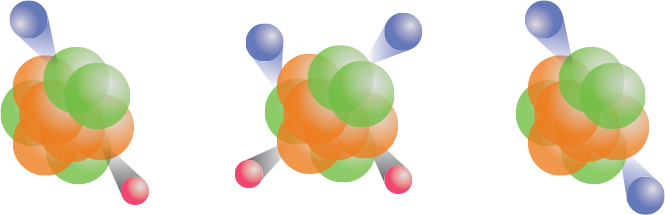
\includegraphics[width=0.6\textwidth]{bb-artist.png}};

    \node[align=center] at (-3.5,-1.9) {\scshape $\upbeta$ decay};
    \node[align=center] at ( 0.0,-1.9) {\scshape double-$\upbeta$ decay};
    \node[align=center] at ( 3.5,-1.9) {\scshape neutrinoless \\ \scshape double-$\upbeta$ decay};

    \node at (-4.3, 1.5) {$e^-$};
    \node at (-2.2,-1.1) {\footnotesize $\overline{\upnu}_e$};

    \node at (-1.2, 1.1) {$e^-$};
    \node at ( 1.4, 1.2) {$e^-$};
    \node at ( 1.3,-1.0) {\footnotesize $\overline{\upnu}_e$};
    \node at (-1.5,-0.9) {\footnotesize $\overline{\upnu}_e$};

    \node at ( 3.2, 1.5) {$e^-$};
    \node at ( 4.6,-1.2) {$e^-$};
  \end{tikzpicture}
\end{center}
In addition to be inevitably tied to the origins of the neutrino mass, neutrinoless
double-beta decay has a second critical consequence on the fundamental laws of Nature. One
of the crucial conserved symmetries in the Standard Model concerns matter and anti-matter:
in all processes they must be produced or destroyed in the same amount.  The world we
know, however, is evidently made of matter --- and cosmological observations seem to
confirm that the rest of the universe looks very similar. How can it be that all the
balancing anti-matter predicted by the Standard Model is gone? The reader might have
realized now, that only matter is produced in neutrinoless double-beta decay.

% vim: tw=90
